\subsection{dataPreservation}
\label{ss:dataPreservation}
Dieses Package beinhaltet die beiden Klassen dieses Projekts welche sich mit dem Schreiben und lesen von Dateien auseinandersetzen. Die Loader Klasse ist hierbei zur Speicherung / zum Laden des Spiels gedacht, w"ahrend sich die Logger Klasse mit dem Schreiben in die Log-Datei besch"aftigt. 

\begin{figure}
	\centering
	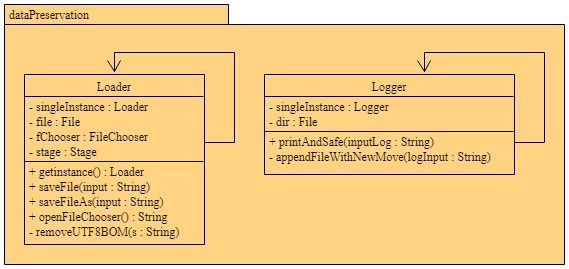
\includegraphics{pics/dataPreservationPackage}
	\caption{UML-Darstellung des dataPreservation packages}
	\label{fig:dataPreservationPackage}
\end{figure}

\paragraph{Singleton-Muster}
\cite{Freeman2006}

\paragraph{Logger}
\label{par:logger}



\paragraph{Loader}
\label{par:loader}



